%
% Class document definition
%
\documentclass[msc]{template/ppgccufmg}  % [phd] | [msc]



%
% Document used packages
%
\usepackage[brazil]{babel}
\usepackage[utf8]{inputenc}
\usepackage[T1]{fontenc}
\usepackage{type1ec}
\usepackage{graphicx}
\usepackage[a4paper,
      portuguese,
      bookmarks=true,
      bookmarksnumbered=true,
      linktocpage,
      colorlinks,
      citecolor=black,
      urlcolor=black,
      linkcolor=black,
      filecolor=black,
]{hyperref}
\usepackage[square]{natbib}
\usepackage{multirow}
\usepackage[usenames,dvipsnames]{xcolor} 


\hyphenation{re-qui-si-to}

\sloppy



%
% The document body and structure
%
\begin{document}



% Definitions for ppgccufmg class
\ppgccufmg{
    title={Grafos como uma primitiva do plano de controle para análise e 
        gerenciamento de Redes Definidas por Software},
    authorrev={Pantuza, Gustavo},
    cutter={M1234x}, % INFORMAÇÃO QUE VAI NA FICHA CATALOGRÁFICA
    cdu={100.0*01.10},  % Define o identificador CDU do documento, fornecido pela Secretaria do Curso.
    university={Universidade Federal de Minas Gerais},
    course={Ciência da Computação},
    address={Belo Horizonte},
    date={2015-03},
    keywords={Redes definidas por software, Openflow, Grafos, 
        Gerenciamento de redes, Sistemas distribuídos, Redes de computadores},
    advisor={Luiz Filipe Menezes Vieira},
    abstract=[brazil]{Resumo}{src/abstract_pt},
    abstract=[english]{Abstract}{src/abstract_en},
    %abstract=[brazil]{Resumo Estendido}{resumoest}, %resumoest.tex
    %dedication={dedicatoria},
    %ack={agradecimentos},
    %  ack=[Acknowledgments]{ack},
    epigraphtext={Live long and prosper!}{Mr. Spock},
}




% Chapters and files that compose the document content
%
% Introduction
%
\section{Introdução}


%
% Community emvolvment
%
\begin{frame}\frametitle{Apresentação}

	\begin{figure}[h]
        \centering
        
\includegraphics[scale=0.5]{images/community.png}
    \end{figure}
\end{frame}


%
% Motivation
%
\begin{frame}\frametitle{Motivação}
   
    \begin{itemize}
        \setlength{\itemsep}{1cm}
        \item A Internet demanda que a infraestrutura evolua em paralelo com 
            as aplicações e serviços
        \item Algoritmos em grafos são base para diversas aplicações em rede
        \item Computação feita em diferentes nós da rede repetidamente
        \item Logicamente centralizado, o plano de controle permite 
            minimizar a quantidade de computações
    \end{itemize}
\end{frame}


%
% Problem
%
\begin{frame}\frametitle{Problema}
    \begin{itemize}
        \setlength{\itemsep}{1cm}
        \item Uma visão topológica global é um dos principais aspectos do 
              paradigma das Redes definidas por software.
        \item Grafos representam de maneira natural e precisa a topologia 
            de uma rede.
        \item Grafos deveriam ser um recurso básico, uma premissa em 
            controladores SDN
    \end{itemize} 
\end{frame}


%
% Scientific contributions
%
\begin{frame}\frametitle{Contribuições científicas}
    \begin{itemize}
        \setlength{\itemsep}{1cm}
        \item Uma abstração da rede na forma de um grafo dinamicamente 
            atualizado.
        \item Avaliações do controlador, da rede e do protocolo OpenFlow
        \item Avaliação de grafos como primitiva em SDN
    \end{itemize}
\end{frame}


\section{Fundamentação teórica}

\section{SDN}



%
% SDN
%
\begin{frame}\frametitle{SDN}

    \begin{itemize}
    \item SDN é apenas um modelo
    \vspace*{0.5cm}
    \item Um \emph{design} para construção e administração de redes
    \vspace*{0.5cm}
    \item A separação dos planos de controle e de dados torna o 
          funcionamento da rede mais flexível
    \end{itemize}
\end{frame}

%
% SDN
%
\begin{frame}\frametitle{Características}

    \begin{itemize}
    \item Torna a rede programável
    \vspace*{0.1cm}
    \item Flexibilidade na administração da rede
    \vspace*{0.1cm}
    \item Controle logicamente centralizado
    \vspace*{0.1cm}
    \item Configurável via programação
    \vspace*{0.1cm}
    \item Padronização aberta 
    \end{itemize}
\end{frame}


%
% Openflow
%
\begin{frame}\frametitle{Openflow}

    \begin{itemize}
    \item Se SDN é só um modelo, como implementá-lo?
    \end{itemize}
    	\begin{figure}[h]
        \centering
        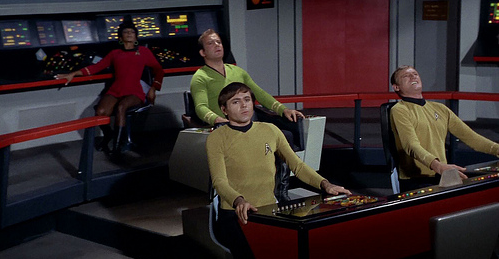
\includegraphics[scale=0.5]{images/control-room.png}
    \end{figure}
\end{frame}



%
% Openflow
%
\begin{frame}\frametitle{Openflow}

    \begin{itemize}
    \item Openflow é um protocolo que possibilita experimentos e aplicações
          em SDN
    \end{itemize}
    	\begin{figure}[h]
        \centering
        
\includegraphics[scale=0.3]{images/openflow.png}
    \end{figure}
\end{frame}


%
% Openflow
%
\begin{frame}\frametitle{Openflow}

    \begin{itemize}
    \item \href{http://archive.openflow.org/documents/openflow-wp-latest.pdf}{Artigo} publicado em 2008 
    \item Permitiu que pesquisadores pudessem criar experimentos com novos
          protocolos em redes convencionais 
    \end{itemize}

\end{frame}




%
% Openflow
%
\begin{frame}\frametitle{Porque é tão importante?}

    \begin{itemize}
    \item A arquitetura da Internet tem deficiências
    \item Inovações em rede custam caro
    \item A arquitetura continua acoplada à infraestrutura
    \item O Openflow define um padrão que qualquer fabricante de     
          \emph{hardware} de rede pode implementar
    \end{itemize}

\end{frame}


\subsection{O protocolo OpenFlow}


%
% Openflow
%
\begin{frame}\frametitle{Openflow}

    \begin{itemize}
    \item Openflow é um protocolo que possibilita experimentos e aplicações
          em SDN
    \end{itemize}
    \begin{figure}[h]
        \centering
        
\includegraphics[scale=0.2]{images/openflow}
    \end{figure}
\end{frame}


%
% Openflow
%
\begin{frame}\frametitle{Openflow}

    \begin{itemize}
        \setlength{\itemsep}{.5cm}
    \item \href{http://archive.openflow.org/documents/openflow-wp-latest.pdf}
        {OpenFlow: Enabling Innovation in Campus Networks} publicado em 2008 
    \item Permitiu que pesquisadores criassem experimentos com novos
          protocolos em redes convencionais.
    \end{itemize}

\end{frame}




%
% Openflow
%
\begin{frame}\frametitle{Definição}

    \begin{itemize}
        \setlength{\itemsep}{.5cm}
        \item Consiste em uma interface de programação para o \emph{switch}
        \item A interface separa de maneira clara os planos de dados e de 
            controle
        \item Um programador pode, através de um programa, controlar a
            forma como um \emph{switch} executa seu encaminhamento de pacotes
        \item O OpenFlow foi criado como um padrão aberto
    \end{itemize}
\end{frame}


%
% Openflow
%
\begin{frame}\frametitle{Componentes}
    Na arquitetura estabelecida pelo protocolo OpenFlow existem dois papéis
    principais.

    \begin{figure}[h]
        \centering
        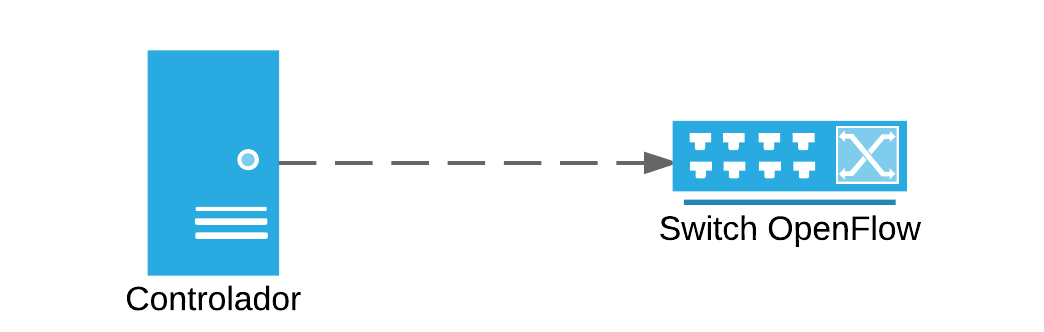
\includegraphics{images/controller-secure-switch}
        \caption{Da esquerda pra direita, plano de controle e plano de dados}
    \end{figure}

\end{frame}


%
% Openflow
%
\begin{frame}\frametitle{Arquitetura OpenFlow}

    \begin{figure}[h!]
        \centering
        \label{fig:switch-arch}
        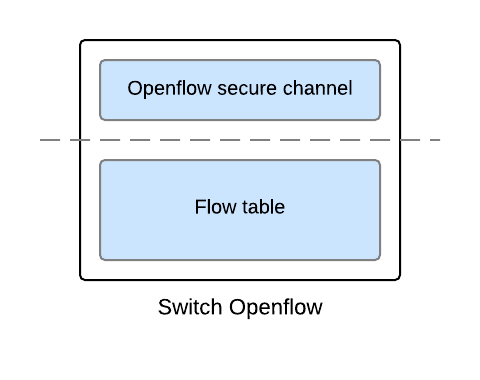
\includegraphics[width=\linewidth]{images/switch-architecture}
        \caption{Arquitetura do comutador OpenFlow}
    \end{figure}

\end{frame}



%
% Switch Archtecture
%
\begin{frame}\frametitle{Arquitetura Openflow}

    \begin{itemize}
        \setlength{\itemsep}{.5cm}
    \item \textbf{Canal seguro OpenFlow}: É a conexão segura entre o
          controlador e o switch openflow
    \item \textbf{Tabela de fluxos}: É a tabela onde são identificados os fluxos
    \item Para cada fluxo tem-se uma ação (action) a ser tomada
    \end{itemize}
\end{frame}


%
% Switch Archtecture
%
\begin{frame}\frametitle{Tabela de fluxos}
    \begin{table}[h!]
    \small
    \centering
    \begin{tabular}{ | l | l | l | l |}
    \hline
    \textbf{Cabeçalho} & \textbf{Contadores} & \textbf{Ações} &
    \textbf{Prioridade} 
    \\ \hline porta de ingresso=5 & 55635 bytes & \pbox{20cm}{Encaminhar 
    \\ porta=8} 
    & 100 \\ \hline
    \pbox{20cm}{Endereço ip=192.168.1.42 \\ porta=80} & 4032 bytes &
    \pbox{30cm}{Rescrita \\ ip=192.168.1.100} & 500 \\ 
    \hline Protocolo IP=UDP & 100 bytes 
    & Drop & 700 \\ \hline
    \end{tabular}
    \caption{Tabela de fluxos simplificada}
    \label{tbl:flowtable}
\end{table}

\end{frame}

%
% Switch Archtecture
%
\begin{frame}\frametitle{Cabeçalho OpenFlow}

    \begin{itemize}
    \item Um fluxo é identificado pelos seguintes campos do cabeçalho 
          Openflow:
    \end{itemize}
	\begin{figure}[h]\hspace*{-1.2cm}
        \centering
        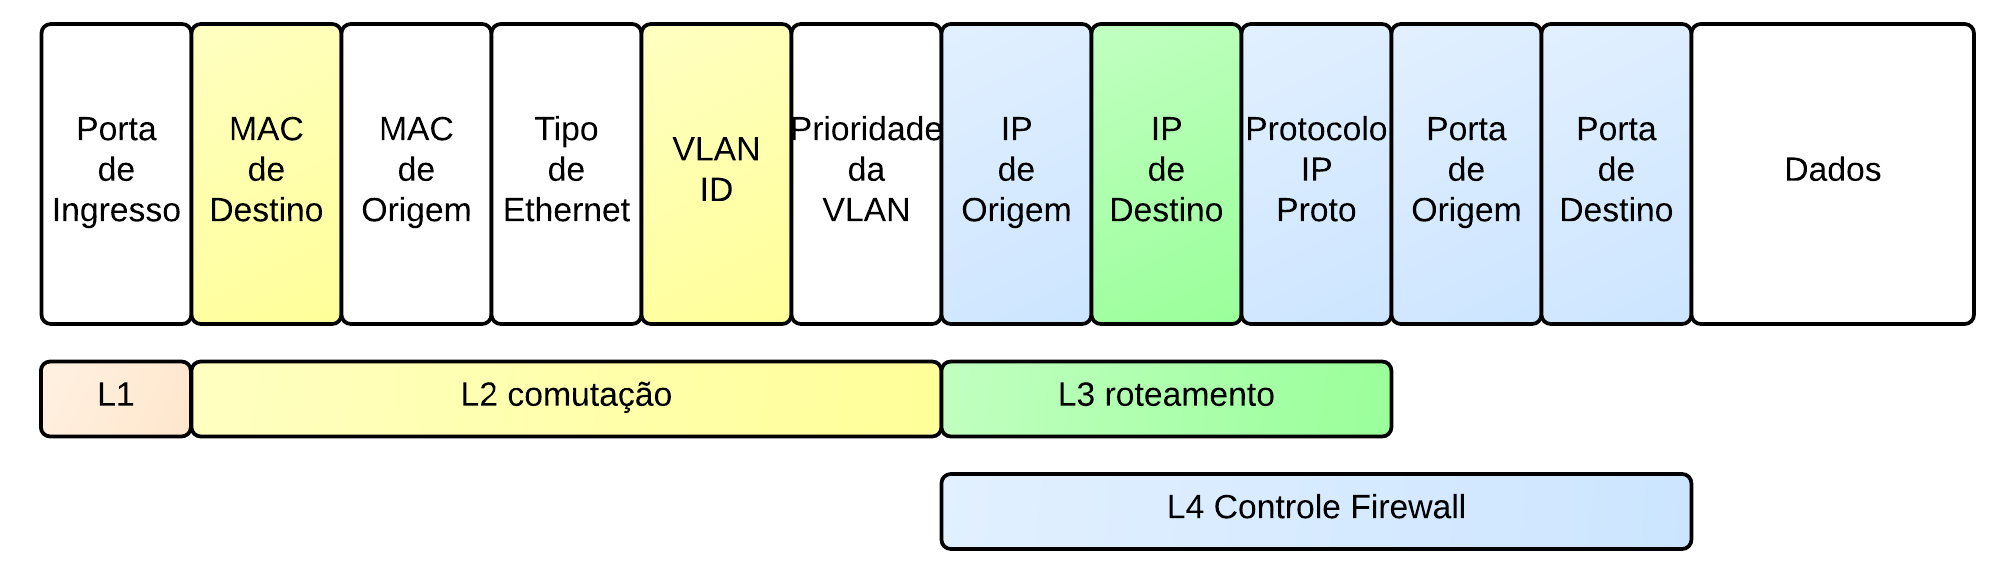
\includegraphics[width=\linewidth]{images/openflow-header}
    \end{figure}
\end{frame}



%
% Actions
%
\begin{frame}\frametitle{Ações}

	\begin{figure}[h]
        \centering
        
\includegraphics[scale=0.5]{images/action.png}
    \end{figure}
    
\end{frame}


%
% Actions
%
\begin{frame}\frametitle{Tipos de ações}

    \begin{columns}[T] % align columns
        \begin{column}{.33\textwidth}

            \begin{itemize}
                \item Forwarding
                \item Drop
                \item Set
                \item strip
                \item Copy-in
                \item Copy-out
                \item Push
                \item Pop
                \item Dec
            \end{itemize}
        \end{column}%
        \hfill%
        \begin{column}{.67\textwidth}
            \begin{figure}[!htb]
                \centering
                
\includegraphics[scale=0.5]{images/action-types}
            \end{figure}
        \end{column}%
    \end{columns}

\end{frame}


%
% Controller
%
\begin{frame}\frametitle{Controlador}

    \begin{itemize}
        \setlength{\itemsep}{.5cm}
    \item É um software que se conecta de maneira segura ao switch openflow
          com o objetivo de manipular sua tabela de fluxos
    \item Esse software pode ser distribuído
    \item Ele representa uma entidade lógica e centralizada
    \item Permite que outros programas troquem mensagens com o 
        plano de controle da rede
    \item Pode calcular estatísticas da rede
    \end{itemize}

\end{frame}


%
% Controller
%
\begin{frame}\frametitle{Controlador}

    \begin{itemize}
    \item Cabe ao programador lidar com os problemas típicos em 
          desenvolvimento de software:
          \begin{itemize}
          \item Tolerância a falha
          \item Persistência
          \item Eficiência
          \item Projeto/design de implementação
          \item debugging
          \item Testes
          \end{itemize}
    \end{itemize}
\end{frame}


%
% Controller
%
\begin{frame}\frametitle{Controlador}

    \begin{itemize}
    \item Controladores Openflow:
          \begin{itemize}
          \item Biblioteca \href{http://opennetworkingfoundation.github.io/libfluid/index.html}{Libfluid}
                para criação de aplicações/controladores em SDN
          \item \href{http://www.noxrepo.org/nox/about-nox/}{Nox Controller}
          \item \href{https://openflow.stanford.edu/display/Beacon/Home}{Beacon}
          \item \href{http://www.noxrepo.org/pox/about-pox/}{Pox Controller}
          \item \href{http://osrg.github.io/ryu/}{Ryu}
          \end{itemize}
    \end{itemize}
\end{frame}

\section{architecture}


%
% Archtecture
%
\begin{frame}\frametitle{Arquitetura Openflow}

    \begin{itemize}
    \item Temos dois papeis principais:
        \begin{itemize}
        \item Controlador
        \item Switch Openflow
        \end{itemize}
    \item Algo te lembra plano de dados e controle desacoplados?
    \end{itemize}
    
	\begin{figure}[h]
        \centering
        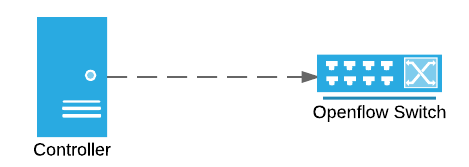
\includegraphics[scale=0.6]{images/controller-to-openflow.png}
    \end{figure}
\end{frame}



%
% Switch Archtecture
%
\begin{frame}\frametitle{Arquitetura do Switch Openflow}

    \begin{itemize}
    \item Internamente um Switch openflow é assim:
    \end{itemize}
    
	\begin{figure}[h]
        \centering
        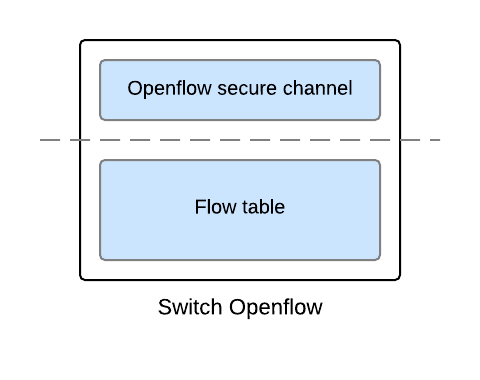
\includegraphics[scale=0.5]{images/openflow-switch-architecture.png}
    \end{figure}
\end{frame}

%
% Switch Archtecture
%
\begin{frame}\frametitle{Arquitetura Openflow}

    \begin{itemize}
    \item \textbf{Openflow secure channel}: É a conexão segura entre o
          controlador e o switch openflow
    \vspace*{0.5cm}
    \item \textbf{Flow table}: É a tabela onde são identificados os fluxos
    \vspace*{0.5cm}
    \item Para cada fluxo tem-se uma ação (action) a ser tomada
    \end{itemize}
\end{frame}

%
% Switch Archtecture
%
\begin{frame}\frametitle{Arquitetura Openflow}

    \begin{itemize}
    \item Um fluxo é identificado pelos seguintes campos do cabeçalho 
          Openflow:
    \end{itemize}
	\begin{figure}[h]\hspace*{-1.2cm}
        \centering
        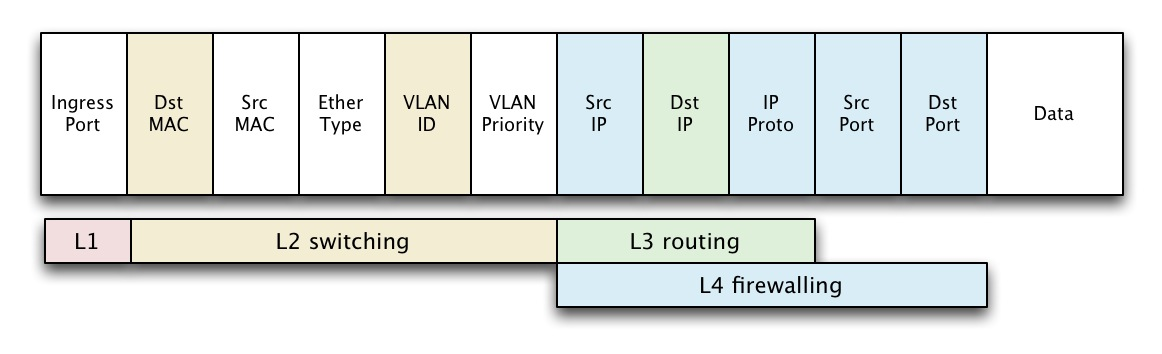
\includegraphics[scale=0.32]{images/openflow-header.jpg}
    \end{figure}
    
\end{frame}


%
% Actions
%
\begin{frame}\frametitle{Actions}

	\begin{figure}[h]
        \centering
        
\includegraphics[scale=0.5]{images/action.png}
    \end{figure}
    
\end{frame}


%
% Actions
%
\begin{frame}\frametitle{Tipos de Actions}

    \begin{itemize}
    \item Forwarding
    \item Drop
    \item Set
    \item strip
    \item Copy-in
    \item Copy-out
    \item Push
    \item Pop
    \item Dec
    \end{itemize}

\end{frame}


%
% Flow table 
%
\begin{frame}\frametitle{Tabela de Fluxos}

\begin{center}
    \begin{tabular}{ | l | l | l | l |}
    \hline
    \textbf{Header} & \textbf{Counters} & \textbf{Actions} & \textbf{Priority} \\ \hline
    in\_port=5 & 55635 bytes & \pbox{20cm}{Forward \\ port=8} & 100 \\ \hline
    \pbox{20cm}{ip=192.168.1.42 \\ port=80} & 4032 bytes & \pbox{30cm}{Set \\ rewrite \\ ip=192.168.1.100} & 500 \\ \hline
    ipproto=UDP & 100 bytes & Drop & 700 \\ \hline
    \end{tabular}
\end{center}

\end{frame}

%
% Controller
%
\begin{frame}\frametitle{Controlador}

    \begin{itemize}
    \item É um software que se conecta de maneira segura ao switch openflow
          com o objetivo de manipular sua tabela de fluxos
    \item Esse software pode ser distribuído
    \item Ele representa uma entidade lógica e centralizada
    \item É possível ter visão e controle de estado global da rede
    \item Permite que outros serviços e programas façam requisições e troca
          de mensagem com o plano de controle da rede
    \item Pode calcular estatísticas da rede
    
    \end{itemize}

\end{frame}


%
% Controller
%
\begin{frame}\frametitle{Controlador}

    \begin{itemize}
    \item Cabe ao programador lidar com os problemas típicos em 
          desenvolvimento de software:
          \begin{itemize}
          \item Tolerância a falha
          \item Persistência
          \item Eficiência
          \item design de implementação
          \item debugging
          \item Testes
          \end{itemize}
    \end{itemize}
\end{frame}

%
% Controller
%
\begin{frame}\frametitle{Controlador}

    \begin{itemize}
    \item Controladores Openflow:
          \begin{itemize}
          \item Biblioteca \href{http://opennetworkingfoundation.github.io/libfluid/index.html}{Libfluid}
                para criação de aplicações/controladores em SDN
          \item \href{http://www.noxrepo.org/nox/about-nox/}{Nox Controller}
          \item \href{https://openflow.stanford.edu/display/Beacon/Home}{Beacon}
          \item \href{http://www.noxrepo.org/pox/about-pox/}{Pox Controller}
          \item \href{http://osrg.github.io/ryu/}{Ryu}
          \end{itemize}
    \end{itemize}
\end{frame}


%
% Simple topology
%
\begin{frame}\frametitle{Arquitetura Openflow}

    \begin{itemize}
    \item Uma topologia simples:
    \end{itemize}
    
	\begin{figure}[h]
        \centering
        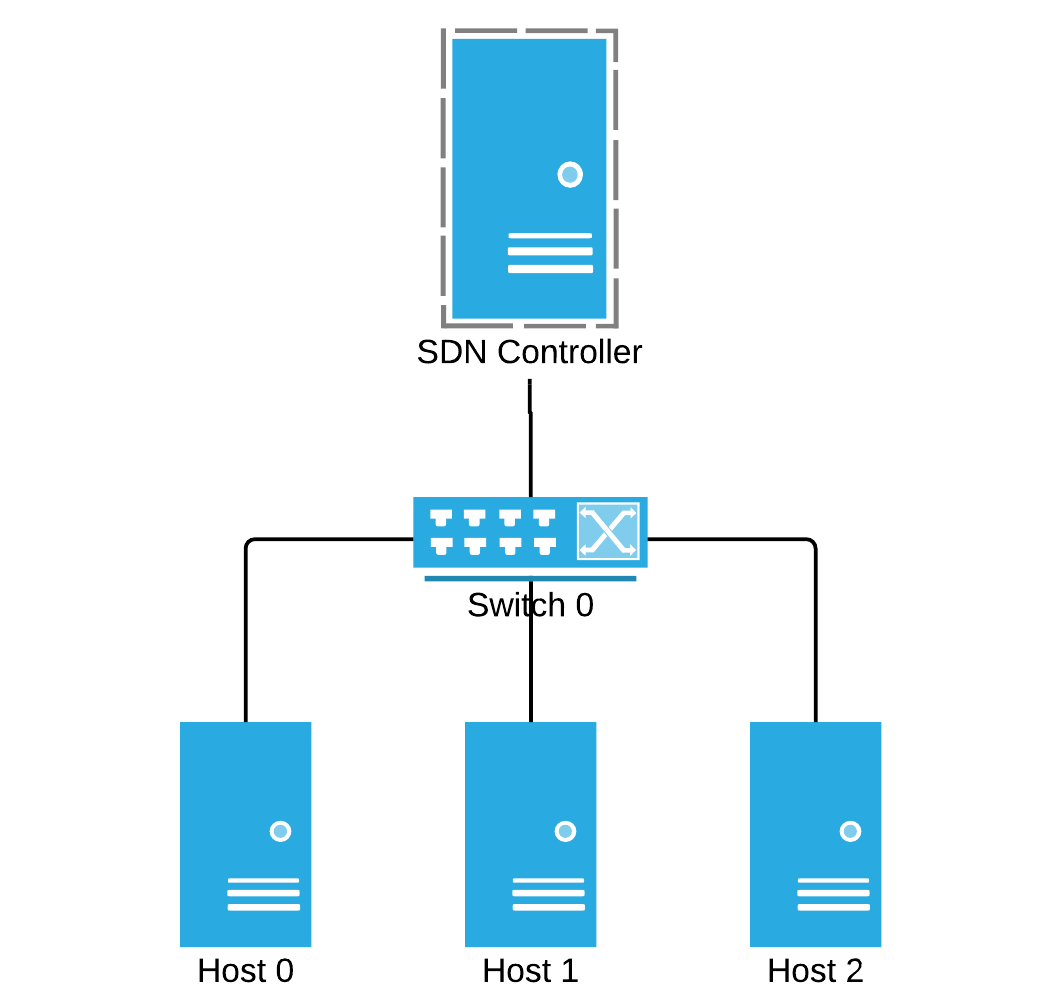
\includegraphics[scale=0.3]{images/simple-topology.png}
    \end{figure}
\end{frame}


%
% N openflow 
%
\begin{frame}\frametitle{Arquitetura Openflow}

    \begin{itemize}
    \item Um controlador para vários \emph{Switches}
    \end{itemize}
    
	\begin{figure}[h]
        \centering
        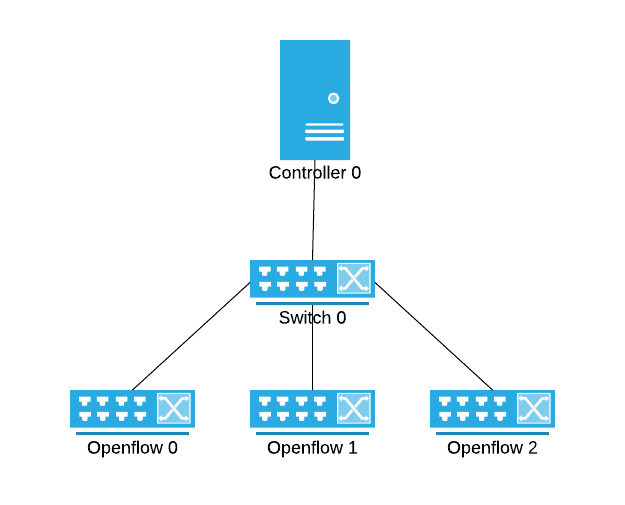
\includegraphics[scale=0.4]{images/n-openflow-switches.png}
    \end{figure}
\end{frame}


%
% SDN inter domain
%
\begin{frame}\frametitle{Arquitetura Openflow}

    \begin{itemize}
    \item Comunicação entre domínios de rede
    \end{itemize}
    
   
	\begin{figure}[h]\hspace*{-1cm}
        \centering
        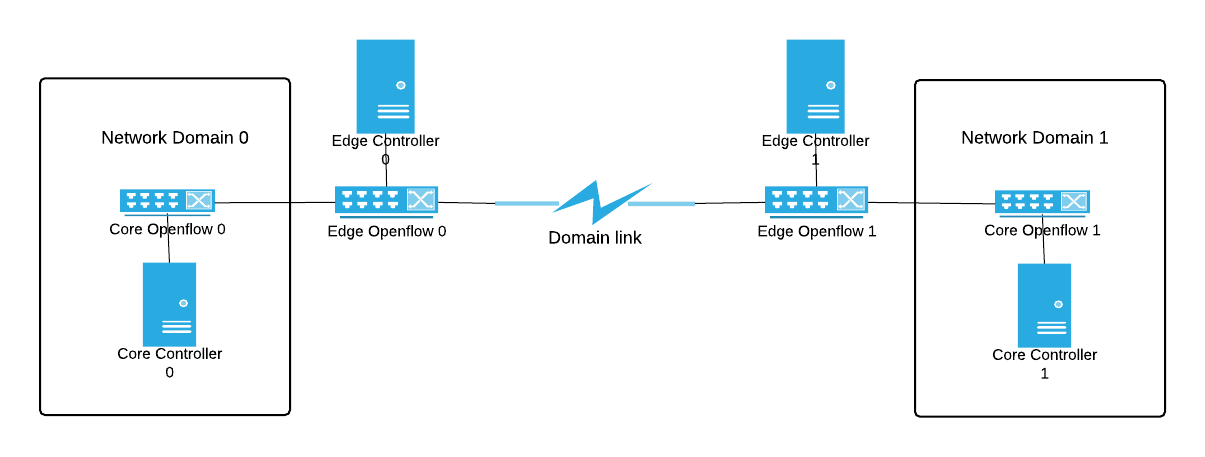
\includegraphics[scale=0.3]{images/edge-core-sdn.png}
    \end{figure}
\end{frame}



%
% Distributed openflow controller
%
\begin{frame}\frametitle{Arquitetura Openflow}

    \begin{itemize}
    \item Controlador distribuído
    \end{itemize}
    
	\begin{figure}[h]
        \centering
        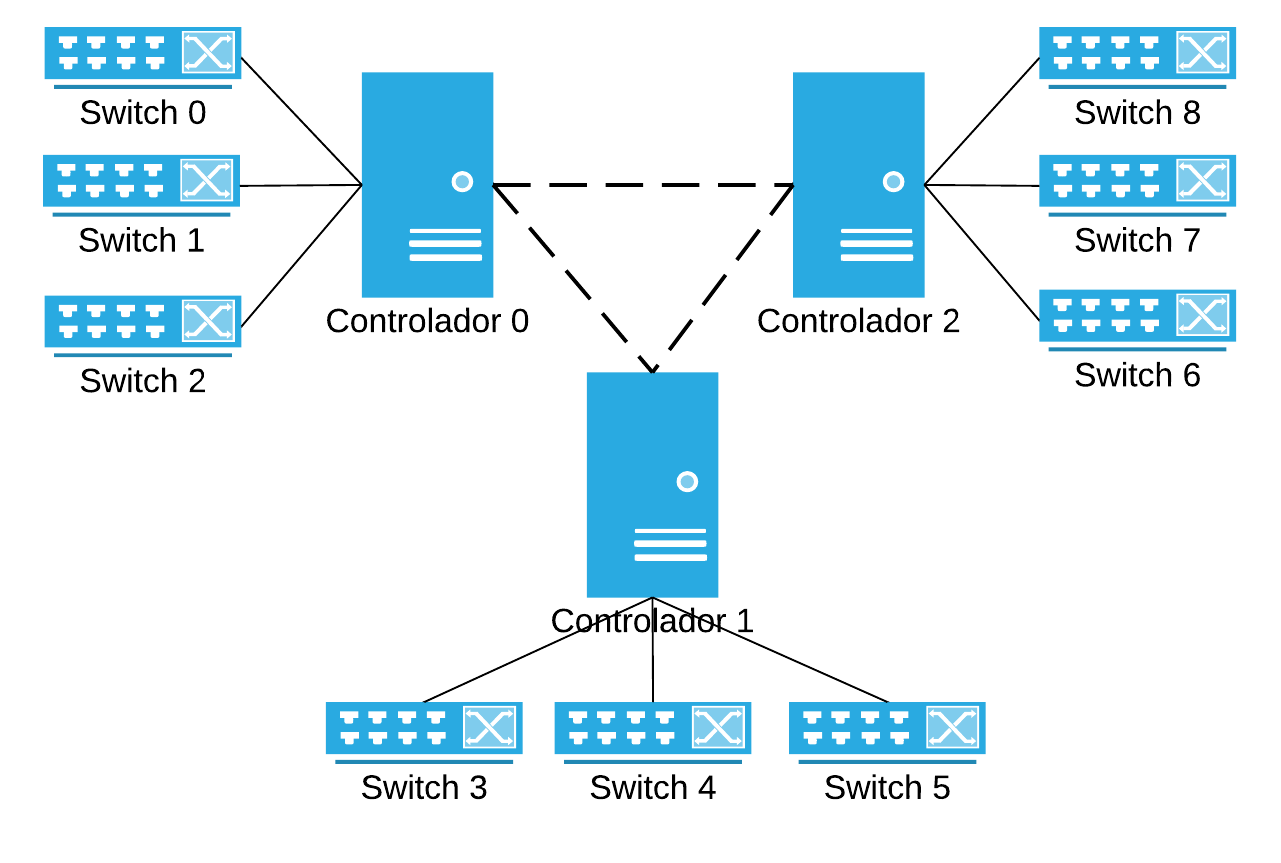
\includegraphics[scale=0.4]{images/distributed_sdn_controller.png}
    \end{figure}
\end{frame}




% Bibliograph file
\ppgccbibliography{src/references}


%\input{apendice} % ARQUIVO CONTENDO OS APÊNDICES : OPCIONAL
%\input{anexo} % ARQUIVO CONTENDO OS ANEXOS: OPCIONAL

\end{document}
